% ---------------------------------------------------------------------------------------------------
\section{Interpretation}
Figure \ref{metrics_all} summarizes the average metrics obtained for each algorithm. While all 
methods show similar accuracy, the logistic regression algorithm shows better results of recall scores 
using oversampled dataset with very small computation time.

\begin{figure}[H]
\centering
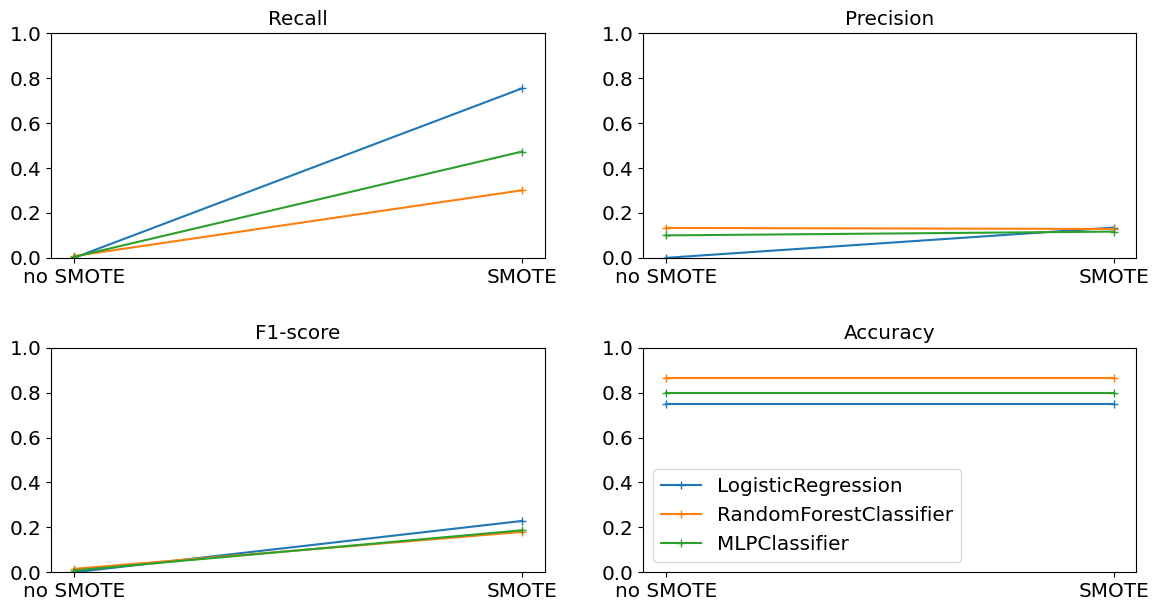
\includegraphics[scale=0.5]{../figures/plot_metrics_all.png}
\caption{Average Recall, Precision, F1-score and Accuracy scores computed for Logistic Regression, 
Random Forest and Multi-Layer Perceptron algorithms using either original dataset sampling (no SMOTE) 
or oversampled dataset (SMOTE).}
\label{metrics_all}
\end{figure}

With an average recall score of 0.76, linear regression models are able to confidently predict true
positive values of stroke. In a medical sudy like this study, one would expect no less than robust 
prediction of true positives.

Prediction scores are always below 0.15 which show that all the models predict a large quantiy of 
false positives. SMOTE application to counteract the class imbalance is insufficient.

With F1-score values lower than 0.3, the models performance is considered as poor.

The accuracy of the models average around 0.8. While this score seems high, in a medical study such 
accuracy might not be sufficient and further analysis or additional dataset inquiry might be 
necessary.\\ 


Out of curiosity, the algorithms have been applied using my personal and medical data. None of the 
models predicts me a risk of stroke. My grand-father died of stroke recently. The logistic regression and 
multi-layer perceptron models whould have predicted him a risk of stroke while the random forest model 
would not predict him any risk of stroke. 
